\begin{figure}[h]
\centering
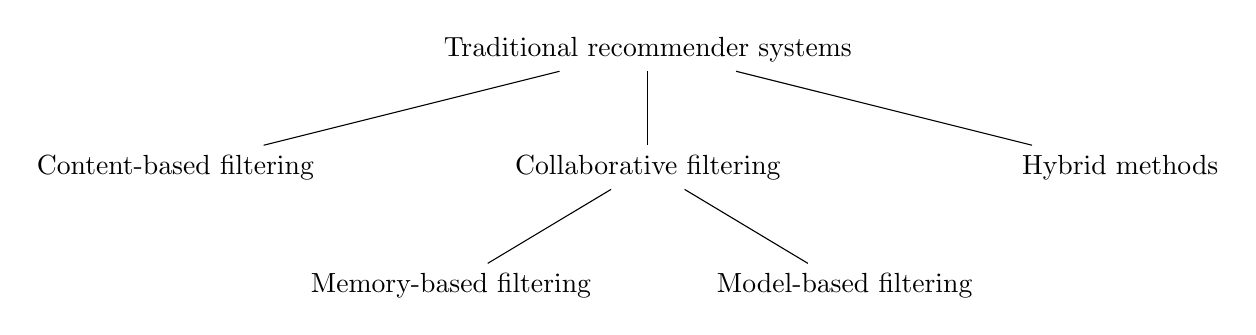
\begin{tikzpicture}[level distance=1.5cm, sibling distance=2.5cm]
\tikzset{
    every node/.style={align=center},
    level 1/.style={sibling distance=6cm},
    level 2/.style={sibling distance=5cm}
}

\node {Traditional recommender systems}
    child {
        node {Content-based filtering}
    }
    child {
        node {Collaborative filtering}
        child {
            node {Memory-based filtering}
        }
        child {
            node {Model-based filtering}
        }
    }
    child {
        node {Hybrid methods}
    };
\end{tikzpicture}

\caption{Types of recommender systems}
\label{fig:RS_taxonomy}
\end{figure}